\begin{problem}{Light Up}{standard input}{standard output}

Light Up(\url{http://www.puzzle-light-up.com/})은 온라인으로 할 수 있는 퍼즐 게임이다. 
이 게임의 규칙은 간단하다. $N \times N$ 크기의 격자판이 주어지는데, 이 격자판의 각 칸은 검정색 정사각형 혹은 흰색 정사각형으로 구성되어 있다. 
이 게임의 목표는 흰색 정사각형에 백열 전구를 아주 잘 놓아, 모든 흰색 정사각형에 불이 들어오게 하는 것이다. 
만약 어떤 흰색 정사각형과 같은 세로줄 혹은 같은 가로줄에 백열 전구가 놓여 있고, 사이에 검정색 정사각형이 없다면 그 흰색 정사각형은 불이 켜진 상태가 된다.

\begin{center}
  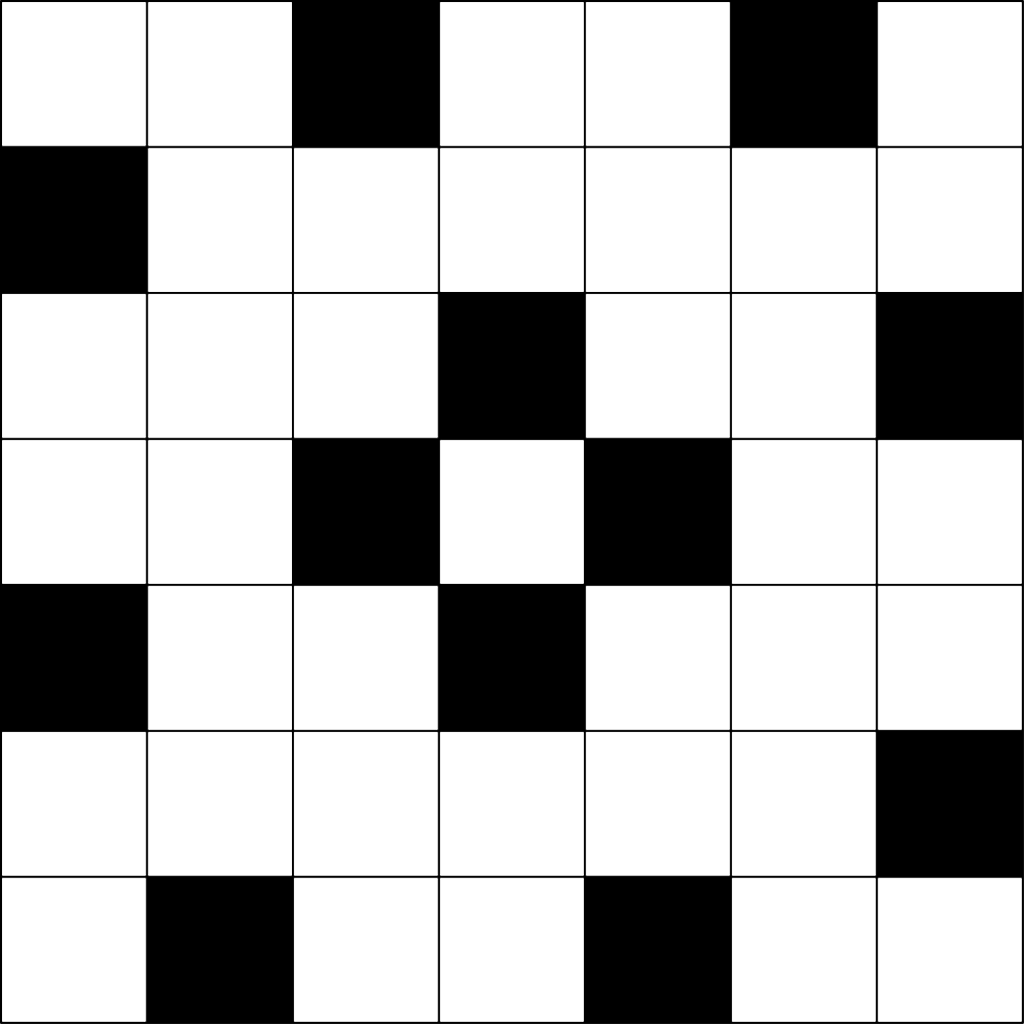
\includegraphics[width=0.35\textwidth]{figure1.png}

  <그림 1>
\end{center}

그림 1과 같은 격자판이 주어졌을 때, ($3, 3$)의 위치에 백열 전구를 배치하면 그림 2와 같은 상황이 된다.

\begin{center}
  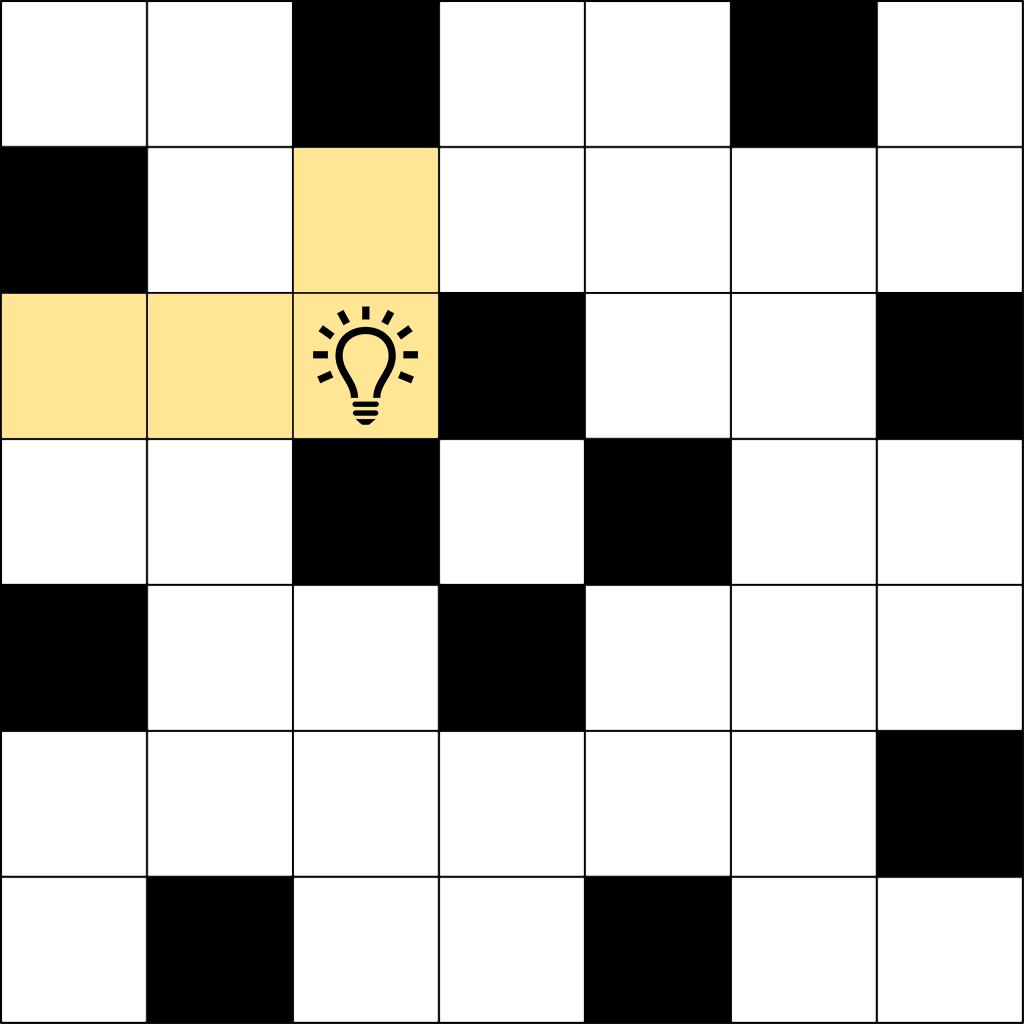
\includegraphics[width=0.35\textwidth]{figure2.png}

  <그림 2>
\end{center}

그런데 이미 불이 켜진 흰색 정사각형에 다른 백열 전구를 놓으면, 백열 전구가 과열되기 때문에 배치를 할 수 없게 된다. 
즉, 그림 3 같이 ($2, 3$)과 ($3, 3$)에 백열 전구를 배치하는 것은 불가능하다.

\begin{center}
  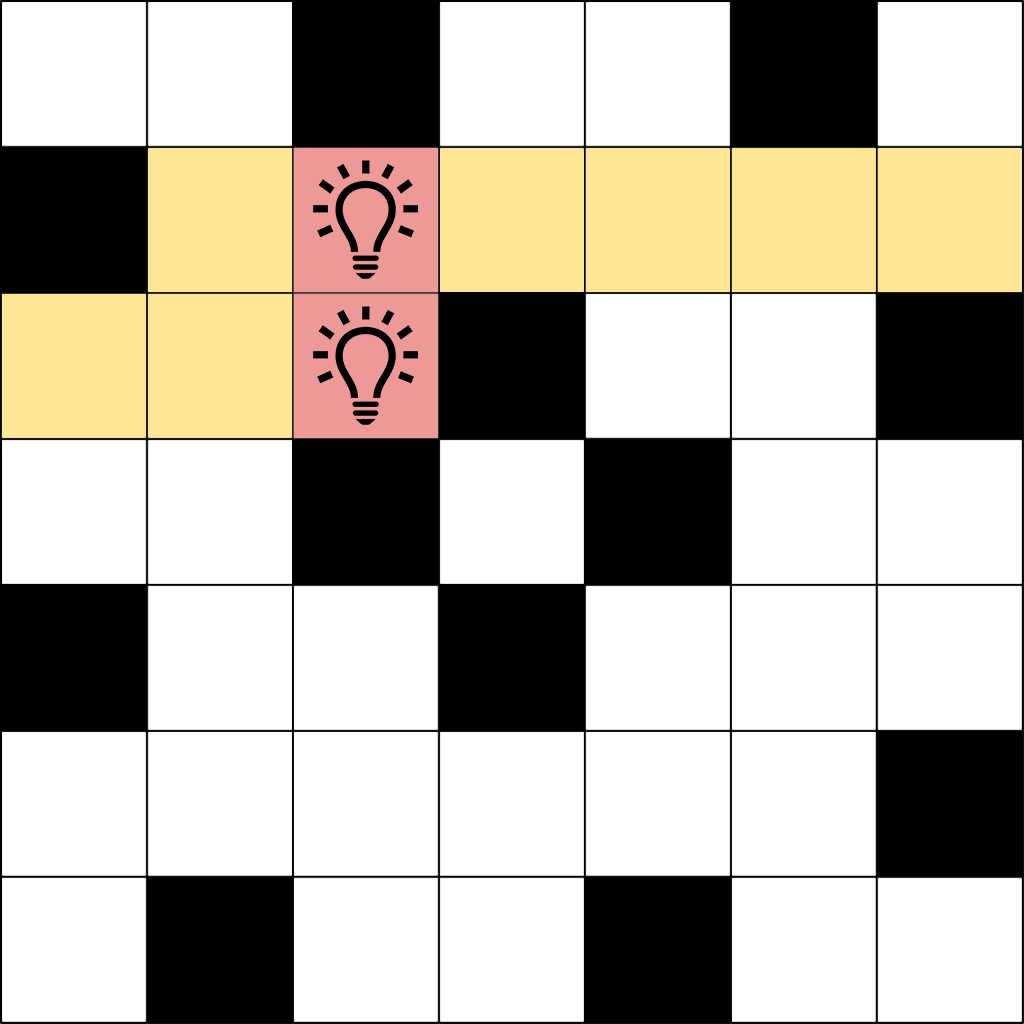
\includegraphics[width=0.35\textwidth]{figure3.png}

  <그림 3>
\end{center}

몇몇 검은 정사각형에는 숫자가 쓰여 있는데, 이는 그 정사각형과 변을 공유하는 네 개의 정사각형 중 백열 전구가 놓여있어야 하는 정사각형의 개수를 의미한다. 
그림 4와 같은 상황을 살펴보자.

\begin{center}
  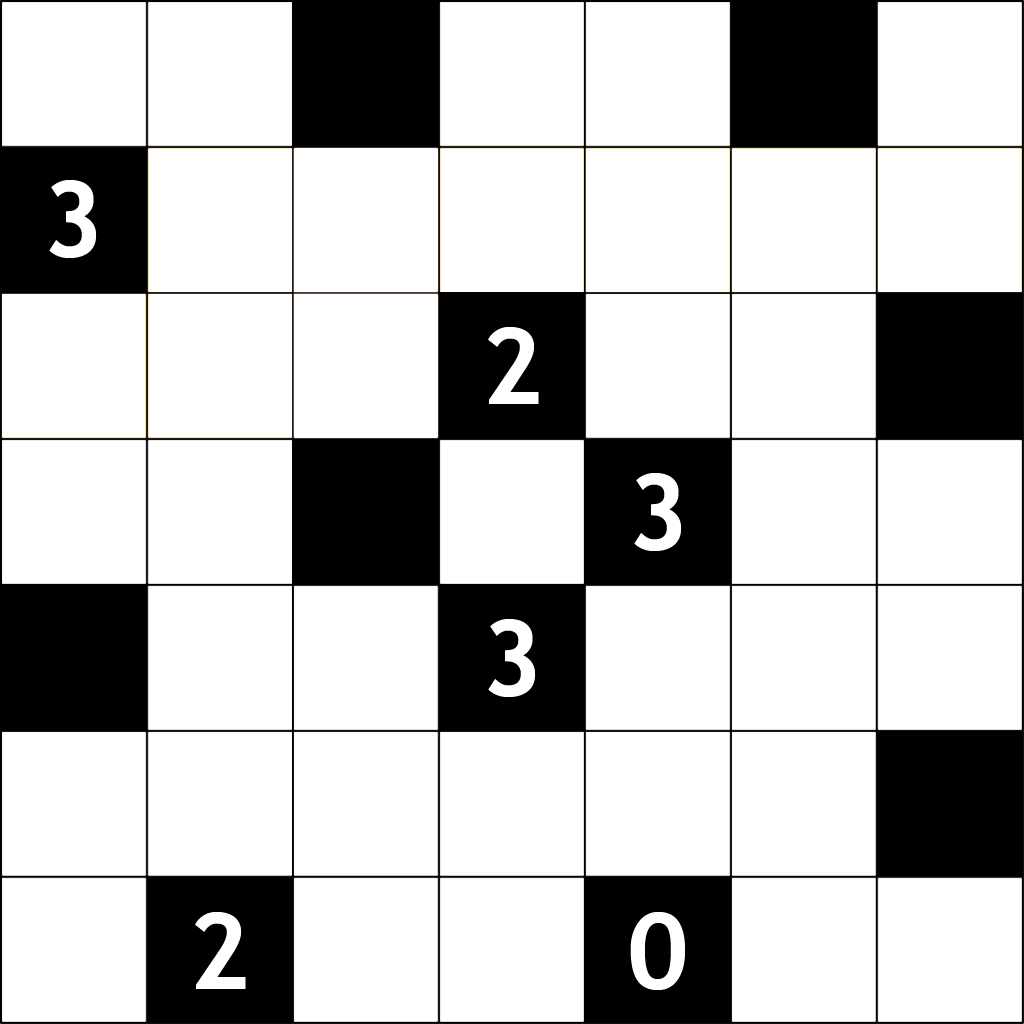
\includegraphics[width=0.35\textwidth]{figure4.png}

  <그림 4>
\end{center}

그림 4와 같은 판이 주어졌을 때, 백열 전구를 잘 배치하는 방법은 그림 5와 같다.

\begin{center}
  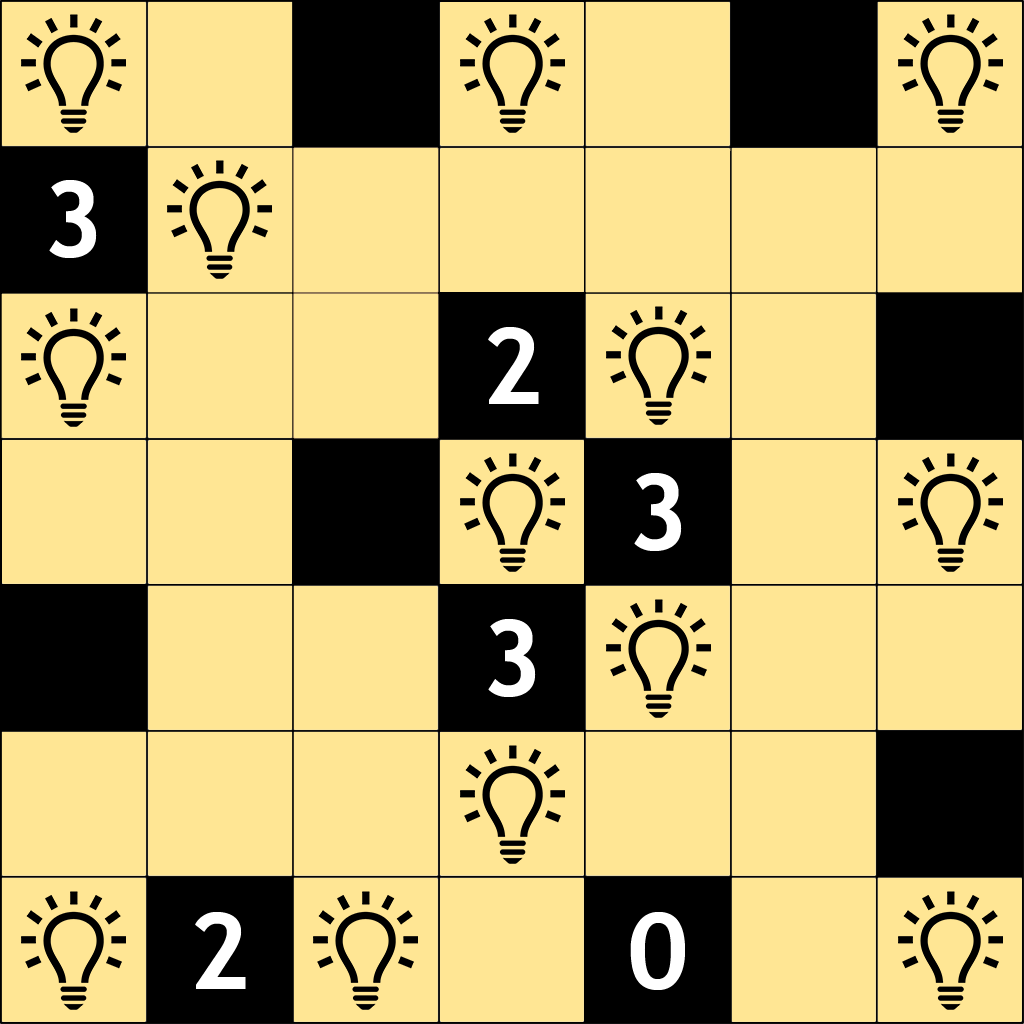
\includegraphics[width=0.35\textwidth]{figure5.png}

  <그림 5>
\end{center}

임의의 격자판이 주어졌을 때, 퍼즐을 해결하는 방법을 알아내자.

\InputFile
첫 번째 줄에 테스트 케이스의 수 $T$가 주어진다. ($1 \le T \le 30$)

테스트 케이스의 첫 번째 줄에 격자판의 크기 $N$이 주어진다. ($1 \le N \le 7$)

테스트 케이스의 두 번째 줄부터 $N$개의 줄에 걸쳐 $N$개의 숫자가 주어진다. 
$i$번째 줄의 $j$번째 숫자는 격자판의 ($i, j$) 위치의 정사각형에 대한 정보 $R_{ij}$이다. 
$R_{ij}$가 $-2$인 경우 흰색 정사각형, $R_{ij}$가 $-1$인 경우 검은색 정사각형, $0$이상 $4$이하인 경우 그 숫자가 적힌 검은색 정사각형이다.

\OutputFile
$N$개의 줄에 걸쳐 각 줄에 $0$ 또는 $1$인 $N$개의 숫자를 출력한다. 
퍼즐을 해결할 수 있도록 백열 전구를 배치한 후, 백열 전구가 배치된 칸은 $1$, 그렇지 않은 칸은 $0$으로 표현하여 출력한다.

답이 항상 존재하는 입력만 주어지고, 두 개 이상의 답이 존재하는 경우 그 중 하나만을 출력한다.

\Example

\begin{example}
\exmp{2
7
-2 -2 -2 -2 -2 0 -2
1 -2 -2 -2 -2 -2 -2
-2 -2 1 -2 2 -2 -2
-2 -2 -2 -2 -2 -2 -2
-2 -2 0 -2 2 -2 -2
-2 -2 -2 -2 -2 -2 2
-2 1 -2 -2 -2 -2 -2
7
-2 -2 -1 -2 -2 -1 -2
3 -2 -2 -2 -2 -2 -2
-2 -2 -2 2 -2 -2 -1
-2 -2 -1 -2 3 -2 -2
-1 -2 -2 3 -2 -2 -2
-2 -2 -2 -2 -2 -2 -1
-2 2 -2 -2 0 -2 -2
}{1 0 0 0 0 0 0
0 0 0 1 0 0 0
0 1 0 0 0 1 0
0 0 0 0 1 0 0
0 0 0 0 0 0 1
0 0 0 0 1 0 0
1 0 0 0 0 0 1
1 0 0 1 0 0 1
0 1 0 0 0 0 0
1 0 0 0 1 0 0 
0 0 0 1 0 0 1
0 0 0 0 1 0 0
0 0 0 1 0 0 0
1 0 1 0 0 0 1
}%
\end{example}

\end{problem}
